%*******************************************************************************
%*********************************** Third Chapter *****************************
%*******************************************************************************

\chapter[Probing Correlations by Global 
  Nondestructive Addressing] {Probing Correlations by Global
  Nondestructive Addressing\footnote{The results of this chapter were
    first published in Ref. \cite{kozlowski2015}}}
\label{chap:qnd}

\ifpdf
    \graphicspath{{Chapter3/Figs/Raster/}{Chapter3/Figs/PDF/}{Chapter3/Figs/}}
\else
    \graphicspath{{Chapter3/Figs/Vector/}{Chapter3/Figs/}}
\fi


%********************************** %First Section  **************************************

\section{Introduction}

Having developed the basic theoretical framework within which we can
treat the fully quantum regime of light-matter interactions we now
consider possible applications. We will first look at nondestructive
measurement where measurement backaction can be neglected and we focus
on what expectation values can be extracted via optical methods.

In this chapter we develop a method to measure properties of ultracold
gases in optical lattices by light scattering. In the previous chapter
we have shown that the quantum light field couples to the bosons via
the operator $\hat{F}$. This is the key element of the scheme we
propose as this makes it sensitive to the quantum state of the matter
and all of its possible superpositions which will be reflected in the
quantum state of the light itself. We have also shown in section
\ref{sec:derivation} that this coupling consists of two parts, a
density component $\hat{D}$ given by Eq. \eqref{eq:D}, and a phase
component $\hat{B}$ given by Eq. \eqref{eq:B}. Therefore, when probing
the quantum state of the ultracold gas we can have access to not only
density correlations, but also matter-field interference at its
shortest possible distance in an optical lattice, i.e.~the lattice
period. Previous work on quantum non-demolition (QND) schemes
\cite{mekhov2007prl, rogers2014, eckert2008} probe only the density
component as it is generally challenging to couple to the matter-field
observables directly. Here, we will consider nondestructive probing of
both density and interference operators.

Firstly, we will consider the simpler and more typical case of
coupling to the atom number operators via $\hat{F} =
\hat{D}$. However, we show that light diffraction in this regime has
several nontrivial characteristics due to the fully quantum nature of
the interaction. Firstly, we show that the angular distribution has
multiple interesting features even when classical diffraction is
forbidden facilitating their experimental observation. We derive new
generalised Bragg diffraction conditions which are different to their
classical counterpart. Furthermore, due to the fully quantum nature of
the interaction our proposal is capable of probing the quantum state
beyond mean-field prediction. We demonstrate this by showing that this
scheme is capable of distinguishing all three phases in the Mott
insulator - superfluid - Bose glass phase transition in a 1D
disordered optical lattice which is not very well described by a
mean-field treatment \cite{cazalilla2011, ejima2011, kuhner2000,
  pino2012, pino2013}. We underline that transitions in 1D are much
more visible when changing an atomic density rather than for
fixed-density scattering. It was only recently that an experiment
distinguished a Mott insulator from a Bose glass via a series of
destructive measurements \cite{derrico2014}. Our proposal, on the
other hand, is nondestructive and is capable of extracting all the
relevant information in a single experiment making our proposal
timely.

Having shown the possibilities created by this nondestructive
measurement scheme we move on to considering light scattering from the
phase related observables via the operator $\hat{F} = \hat{B}$. This
enables in-situ probing of the matter-field coherence at its shortest
possible distance in an optical lattice, i.e. the lattice period,
which defines key processes such as tunnelling, currents, phase
gradients, etc. This is in contrast to standard destructive
time-of-flight measurements which deal with far-field interference
although a relatively near-field scheme was use in
Ref. \cite{miyake2011}. We show how within the mean-field treatment,
this enables measurements of the order parameter, matter-field
quadratures and squeezing. This can have an impact on atom-wave
metrology and information processing in areas where quantum optics
already made progress, e.g., quantum imaging with pixellized sources
of non-classical light \cite{golubev2010, kolobov1999}, as an optical
lattice is a natural source of multimode nonclassical matter waves.

\section{Coupling to the Quantum State of Matter}

As we have seen in section \ref{sec:a} under certain approximations
the scattered light mode, $\a_1$, is linked to the quantum state of
matter via 
\begin{equation}
  \label{eq:a-3}
  \a_1 = C \hat{F} = C \left(\hat{D} + \hat{B} \right),
\end{equation}
where the atomic operators $\hat{D}$ and $\hat{B}$, given by
Eq. \eqref{eq:D} and Eq. \eqref{eq:B}, are responsible for the
coupling to on-site density and inter-site interference
respectively. It is crucial to note that light couples to the bosons
via an operator as this makes it sensitive to the quantum state of the
matter as this will imprint the fluctuations in the quantum state of
the scattered light.

Here, we will use this fact that the light is sensitive to the atomic
quantum state due to the coupling of the optical and matter fields via
operators in order to develop a method to probe the properties of an
ultracold gas. Therefore, we neglect the measurement backaction and
we will only consider expectation values of light observables. Since
the scheme is nondestructive (in some cases, it even satisfies the
stricter requirements for a QND measurement \cite{mekhov2012,
  mekhov2007pra}) and the measurement only weakly perturbs the system,
many consecutive measurements can be carried out with the same atoms
without preparing a new sample. We will show how the extreme
flexibility of the the measurement operator $\hat{F}$ allows us to
probe a variety of different atomic properties in-situ ranging from
density correlations to matter-field interference.

\section{On-site Density Measurements}

\subsection{Diffraction Patterns and Bragg Conditions}

We have seen in section \ref{sec:B} that typically the dominant term
in $\hat{F}$ is the density term $\hat{D}$ \cite{mekhov2007pra,
  LP2009, rist2010, lakomy2009, ruostekoski2009}. This is simply due
to the fact that atoms are localised with lattice sites leading to an
effective coupling with atom number operators instead of inter-site
interference terms. Therefore, we will first consider nondestructive
probing of the density related observables of the quantum
gas. However, we will focus on the novel nontrivial aspects that go
beyond the work in Ref. \cite{mekhov2012, mekhov2007prl,
  mekhov2007pra} which only considered a few extremal cases.

As we are only interested in the quantum information imprinted in the
state of the optical field we will simplify our analysis by
considering the light scattering to be much faster than the atomic
tunnelling. Therefore, our scheme is actually a QND scheme
\cite{mekhov2007prl, mekhov2007pra, rogers2014, eckert2008} as
normally density-related measurements destroy the matter-phase
coherence since it is its conjugate variable, but here we neglect the
$\bd_i b_j$ terms. Furthermore, we will consider a deep
lattice. Therefore, the Wannier functions will be well localised
within their corresponding lattice sites and thus the coefficients
$J_{i,i}$ reduce to $u_1^*(\b{r}_i) u_0(\b{r}_i)$ leading to
\begin{equation}
  \label{eq:D-3}
  \hat{D}=\sum_i^K u_1^*(\b{r}_i) u_0(\b{r}_i) \hat{n}_i,
\end{equation} 
which for travelling
[$u_l(\b{r})=\exp(i \b{k}_l \cdot \b{r}+i\varphi_l)$] or standing
[$u_l(\b{r})=\cos(\b{k}_l \cdot \b{r}+\varphi_l)$] waves is just a
density Fourier transform at one or several wave vectors
$\pm(\b{k}_1 \pm \b{k}_0)$. 

We will now define a new auxiliary quantity to aid our analysis,
\begin{equation}
  \label{eq:R}
  R = \langle \ad_1 \a_1 \rangle - | \langle \a_1 \rangle |^2,
\end{equation}
which we will call the ``quantum addition'' to light scattering. By
construction $R$ is simply the full light intensity minus the
classical field diffraction. In order to justify its name we will show
that this quantity depends purely quantum mechanical properties of the
ultracold gas. We substitute $\a_1 = C \hat{D}$ using
Eq. \eqref{eq:D-3} into our expression for $R$ in Eq. \eqref{eq:R} and
we make use of the shorthand notation
$A_i = u_1^*(\b{r}_i) u_0(\b{r}_i)$. The result is
\begin{equation}
  \label{eq:Rfluc}
  R = |C|^2 \sum_{i,j}^K A^*_i A_j \langle \delta \hat{n}_i \delta
  \hat{n}_j \rangle,
\end{equation}
where $\delta \hat{n}_i = \hat{n}_i - \langle \hat{n}_i
\rangle$. Thus, we can clearly see that $R$ is a result of light
scattering from fluctuations in the atom number which is a purely
quantum mechanical property of a system. Therefore, $R$, the ``quantum
addition'' faithfully represents the new contribution from the quantum
light-matter interaction to the diffraction pattern.

Another interesting quantity to measure are the quadratures of the
light fields which we have seen in section \ref{sec:a} are related to
the quadrature of $\hat{F}$ by $\hat{X}_\phi = |C|
\hat{X}^F_\beta$. An interesting feature of quadratures is that the
coupling strength at different sites can be tuned using the local
oscillator phase $\beta$. To see this we consider the case when both
the scattered mode and probe are travelling waves the quadrature
\begin{equation} 
  \label{eq:Xtrav}
  \hat{X}^F_\beta = \frac{1}{2} \left( \hat{F} e^{-i \beta} +
    \hat{F}^\dagger e^{i \beta} \right) = \sum_i^K \hat{n}_i\cos[(\b{k}_0 - \b{k}_1) \cdot
  \b{r}_i + (\phi_0 - \phi_1) - \beta].
\end{equation} 
Different light quadratures are differently coupled to the atom
distribution, hence by varying the local oscillator phase, $\beta$,
and/or the detection angle one can scan the whole range of
couplings. This is similar to the case for $\hat{D}$ for a standing
wave probe, where instead of varying $\beta$ scanning is achieved by
varying the position of the wave with respect to atoms. Additionally,
the quadrature variance, $(\Delta X^F_\beta)^2$, will have a similar
form to $R$ given in Eq. \eqref{eq:Rfluc},
\begin{equation}
  (\Delta X^F_\beta)^2 = |C|^2 \sum_{i.j}^K A_i^\beta A_j^\beta
  \langle \dn_i \dn_j \rangle,
\end{equation}
where $A_i^\beta = (A_i e^{-i\beta} + A_i^* e^{i \beta})/2$.  However,
this has the advantage that unlike in the case of $R$ there is no need
to subtract a spatially varying classical signal to obtain this
quantity.

The ``quantum addition'', $R$, and the quadrature variance,
$(\Delta X^F_\beta)^2$, are both quadratic in $\a_1$ and both rely
heavily on the quantum state of the matter. Therefore, they will have
a nontrivial angular dependence showing more peaks than classical
diffraction. Furthermore, these peaks can be tuned very easily with
$\beta$ or $\varphi_l$. Fig. \ref{fig:scattering} shows the angular
dependence of $R$ for the case when the probe is a travelling wave
scattering from an ideal superfluid in a 3D optical lattice into a
standing wave mode. The first noticeable feature is the isotropic
background which does not exist in classical diffraction. This
background yields information about density fluctuations which,
according to mean-field estimates (i.e.~inter-site correlations are
ignored), are related by
$R = |C|^2 K( \langle \hat{n}^2 \rangle - \langle \hat{n} \rangle^2
)/2$. In Fig. \ref{fig:scattering} we can see a significant signal of
$R = |C|^2 N_K/2$, because it shows scattering from an ideal
superfluid which has significant density fluctuations with
correlations of infinte range. However, as the parameters of the
lattice are tuned across the phase transition into a Mott insulator
the signal goes to zero. This is because the Mott insulating phase has
well localised atoms at each site which suppresses density
fluctuations entirely leading to absolutely no ``quantum addition''.

\begin{figure}
  \centering
  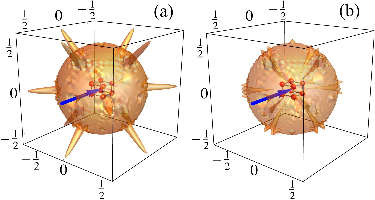
\includegraphics[width=0.8\linewidth]{Ep1}
  \caption[Light Scattering Angular Distribution]{Light intensity
    scattered into a standing wave mode from a superfluid in a 3D
    lattice (units of $R/(|C|^2N_K)$). Arrows denote incoming
    travelling wave probes. The classical Bragg condition,
    $\Delta \b{k} = \b{G}$, is not fulfilled, so there is no classical
    diffraction, but intensity still shows multiple peaks, whose
    heights are tunable by simple phase shifts of the optical beams:
    (a) $\varphi_1=0$; (b) $\varphi_1=\pi/2$. Interestingly, there is
    also a significant uniform background level of scattering which
    does not occur in its classical counterpart. }
  \label{fig:scattering}
\end{figure}

We can also observe maxima at several different angles in
Fig. \ref{fig:scattering}. Interestingly, they occur at different
angles than predicted by the classical Bragg condition. Moreover, the
classical Bragg condition is actually not satisfied which means there
actually is no classical diffraction on top of the ``quantum
addition'' shown here. Therefore, these features would be easy to see
in an experiment as they wouldn't be masked by a stronger classical
signal.  This difference in behaviour is due to the fact that
classical diffraction is ignorant of any quantum correlations as it is
given by the square of the light field amplitude squared
\begin{equation}
  |\langle \a_1 \rangle|^2 = |C|^2 \sum_{i,j} A_i^*
  A_j \langle \n_i \rangle \langle \n_j \rangle,
\end{equation}
which is idependent of any two-point correlations unlike $R$. On the
other hand the full light intensity (classical signal plus ``quantum
addition'') of the quantum light does include higher-order
correlations
\begin{equation}
  \langle \ad_1 \a_1 \rangle = |C|^2 \sum_{i,j} A_i^*
  A_j \langle \n_i \n_j \rangle.
\end{equation}
Therefore, we see that in the fully quantum picture light scattering
not only depends on the diffraction structure due to the distribution
of atoms in the lattice, but also on the quantum correlations between
different lattice sites which will in turn be dependent on the quantum
state of the matter. These correlations are imprinted in $R$ as shown
in Eq. \eqref{eq:Rfluc} and it highlights the key feature of our
model, i.e.~the light couples to the quantum state directly via
operators.

We can even derive the generalised Bragg conditions for the peaks that
we can see in Fig. \ref{fig:scattering}. The exact conditions under
which diffraction peaks emerge for the ``quantum addition'' will
depend on the optical setup as well as on the quantum state of the
matter as it is the density fluctuation correlations,
$\langle \dn_i \dn_j \rangle$, that provide the structure for $R$ and
not the lattice itself as seen in Eq. \eqref{eq:Rfluc}. For classical
light it is straightforward to develop an intuitive physical picture
to find the Bragg condition by considering angles at which the
distance travelled by light scattered from different points in the
lattice is equal to an integer multiple of the wavelength. The
``quantum addition'' is more complicated and less intuitive as we now
have to consider quantum correlations which are not only nonlocal, but
can also be negative.

We will consider scattering from a superfluid, because the Mott
insulator has no ``quantum addition'' due to a lack of density
fluctuations. The wavefunction of a superfluid on a lattice is given
by Eq. \eqref{eq:GSSF}. This state has infinte range correlations and
thus has the convenient property that all two-point density
fluctuation correlations are equal regardless of their separation,
i.e.~$\langle \dn_i \dn_j \rangle \equiv \langle \dn_a \dn_b \rangle$
for all $(i \ne j)$, where the right hand side is a constant
value. This allows us to extract all correlations from the sum in
Eq. \eqref{eq:Rfluc} to obtain
\begin{equation}
  \label{eq:RSF}
  \frac{R}{|C|^2} = (\langle \dn^2 \rangle - \langle \dn_a \dn_b \rangle) \sum_i^K
  |A_i|^2 + \langle \dn_a \dn_b \rangle |A|^2 = \frac{N}{M} \sum_i^K
  |A_i|^2 - \frac{N}{M^2} |A|^2,
\end{equation}
where $A = \sum_i^K A_i$, and we have dropped the index from
$\langle \dn^2 \rangle$ as it is equal at every site. The second
equality follows from the fact that for a superfluid state
$\langle \dn^2 \rangle = N/M - N/M^2$ and
$\langle \dn_a \dn_b \rangle = -N/M^2$. Naturally, we get an identical
expression for the quadrature variance $(\Delta X^F_\beta)^2$ with the
coefficients $A_i$ replaced by the real $A_i^\beta$.

The ``quantum addition'' for the case when both the scattered and
probe modes are travelling waves is actually trivial. It has no peaks
and thus it has no generalised Bragg condition and it only consists of
a uniform background. This is a consequence of the fact that
travelling waves couple equally strongly with every atom as only the
phase is different between lattice sites. Therefore, since superfluid
correlations lack structure as they're uniform we do no get a strong
coherent peak. The contribution from the lattice structure is included
in the classical Bragg peaks which we have subtracted in order to
obtain the quantity $R$. However, if we consider the case where the
scattered mode is collected as a standing wave using a pair of mirrors
we get the diffraction pattern that we saw in
Fig. \ref{fig:scattering}. This time we get strong visible peaks,
because at certain angles the standing wave couples to the atoms
maximally at all lattice sites and thus it uses the structure of the
lattice to amplify the signal from the quantum fluctuations. This
becomes clear when we look at Eq. \eqref{eq:RSF}. We can neglect the
second term as it is always negative and it has the same angular
distribution as the classical diffraction pattern and thus it is
mostly zero except when the classical Bragg condition is
satisfied. Since in Fig. \ref{fig:scattering} we have chosen an angle
such that the Bragg condition is not satisfied this term is
essentially zero. Therefore, we are left with the first term
$\sum_i^K |A_i|^2$ which for a travelling wave probe and a standing
wave scattered mode is
\begin{equation}
  \sum_i^K |A_i|^2 = \sum_i^K \cos^2(\b{k}_0 \cdot \b{r}_i + \phi_0) =
  \frac{1}{2} \sum_i^K \left[1 + \cos(2 \b{k}_0 \cdot \b{r}_i + 2
    \phi_0) \right].
\end{equation}
Therefore, it is straightforward to see that unless
$2 \b{k}_0 = \b{G}$, where $\b{G}$ is a reciprocal lattice vector,
there will be no coherent signal and we end up with the mean uniform
signal of strength $|C|^2 N_k/2$. When this condition is satisifed all
the cosine terms will be equal and they will add up constructively
instead of cancelling each other out. Note that this new Bragg
condition is different from the classical one
$\b{k}_0 - \b{k}_1 = \b{G}$. This result makes it clear that the
uniform background signal is not due to any coherent scattering, but
rather due to the lack of structure in the quantum
correlations. Furthermore, we see that the peak height is actually
tunable via the phase, $\phi_0$, which is illustrated in
Fig. \ref{fig:scattering}b.

For light field quadratures the situation is different, because as we
have seen in Eq. \eqref{eq:Xtrav} even for travelling waves we can
tune the contributions to the signal from different sites by changing
the angle of measurement or tuning the local oscillator signal
$\beta$. The rest is similar to the case we discussed for $R$ with a
standing wave mode and we can show that the new Bragg condition in
this case is $2 (\b{k}_0 - \b{k}_1) = \b{G}$ which is different from
the condition we had for $R$ and is still different from the classical
condition $\b{k}_0 - \b{k}_1 = \b{G}$. Furthermore, just like in
Fig. \ref{fig:scattering}b the peak height can be tuned using $\beta$.

A quantum signal that isn't masked by classical diffraction is very
useful for future experimental realisability. However, it is still
unclear whether this signal would be strong enough to be
visible. After all, a classical signal scales as $N_K^2$ whereas here
we have only seen a scaling of $N_K$. In section \ref{sec:Efield} we
have estimated the mean photon scattering rates integrated over the
solid angle for the only two experiments so far on light diffraction
from truly ultracold bosons where the measurement object was light
\begin{equation} 
  n_{\Phi}= \left(\frac{\Omega_0}{\Delta_a}\right)^2 \frac{\Gamma K}{8}
  (\langle\hat{n}^2\rangle-\langle\hat{n}\rangle^2).
\end{equation} 
These results can be applied directly to the scattering patters in
Fig. \ref{fig:scattering}. Therefore, the background signal should
reach $n_\Phi \approx 10^6$ s$^{-1}$ in Ref. \cite{weitenberg2011}
(150 atoms in 2D), and $n_\Phi \approx 10^{11}$ s$^{-1}$ in
Ref. \cite{miyake2011} ($10^5$ atoms in 3D). These numbers show that
the diffraction patterns we have seen due to the ``quantum addition''
should be visible using currently available technology, especially
since the most prominent features, such as Bragg diffraction peaks, do
not coincide at all with the classical diffraction pattern.

\subsection{Mapping the Quantum Phase Diagram}

We have shown that scattering from atom number operators leads to a
purely quantum diffraction pattern which depends on the density
fluctuations and their correlations. We have also seen that this
signal should be strong enough to be visible using currently available
technology. However, so far we have not looked at what this can tell
us about the quantum state of matter. We have briefly mentioned that a
deep superfluid will scatter a lot of light due to its infinite range
correlations and a Mott insulator will not contribute any ``quantum
addition'' at all, but we have not looked at the quantum phase
transition between these two phases. In two or higher dimensions this
has a rather simple answer as the Bose-Hubbard phase transition is
described well by mean-field theories and it has a sharp transition at
the critical point. This means that the ``quantum addition'' signal
would drop rapidly at the critical point and go to zero as soon as it
was crossed. However, $R$ given by Eq. \eqref{eq:R} clearly contains
much more information.

There are many situations where the mean-field approximation is not a
valid description of the physics. A prominent example is the
Bose-Hubbard model in 1D \cite{cazalilla2011, ejima2011, kuhner2000,
  pino2012, pino2013} as we have seen in section
\ref{sec:BHM1D}. Observing the transition in 1D by light at fixed
density was considered to be difficult \cite{rogers2014} or even
impossible \cite{roth2003}. This is because the one-dimensional
quantum phase transition is in a different universality class than its
higher dimensional counterparts. The energy gap, which is the order
parameter, decays exponentially slowly across the phase transition
making it difficult to identify the phase transition even in numerical
simulations. Here, we will show the avaialable tools provided by the
``quantum addition'' that allows one to nondestructively map this
phase transition and distinguish the superfluid and Mott insulator
phases.

The 1D phase transition is best understood in terms of two-point
correlations as a function of their separation \cite{giamarchi}. In
the Mott insulating phase, the two-point correlations $\langle \bd_i
b_j \rangle$ and $\langle \delta \hat{n}_i \delta \hat{n}_j \rangle$
($\delta \hat{n}_i =\hat{n}_i-\langle \hat{n}_i\rangle$) decay
exponentially with $|i-j|$. This is a characteristic of insulators. On
the other hand the superfluid will exhibit long-range order which in
dimensions higher than one, manifests itself with an infinite
correlation length. However, in 1D only pseudo long-range order
happens and both the matter-field and density fluctuation correlations
decay algebraically \cite{giamarchi}.

The method we propose gives us direct access to the structure factor,
which is a function of the two-point correlation $\langle \delta
\hat{n}_i \delta \hat{n}_j \rangle$. This quantity can be extracted
from the measured light intensity by considering the ``quantum
addition''. We will consider the case when both the probe and
scattered modes are plane waves which can be easily achieved in free
space. We will again consider the case of light being maximally
coupled to the density ($\hat{F} = \hat{D}$). Therefore, the quantum
addition is given by
\begin{equation} 
  R =\sum_{i, j} \exp[i (\mathbf{k}_1 - \mathbf{k}_0)
  (\mathbf{r}_i - \mathbf{r}_j)] \langle \delta \hat{n}_i \delta
  \hat{n}_j \rangle.
\end{equation}

This alone allows us to analyse the phase transition quantitatively
using our method. Unlike in higher dimensions where an order parameter
can be easily defined within the mean-field approximation as a simple
expectation value, the situation in 1D is more complex as it is
difficult to directly access the excitation energy gap which defines
this phase transition. However, a valid description of the relevant 1D
low energy physics is provided by Luttinger liquid theory
\cite{giamarchi} as seen in section \ref{sec:BHM1D}. In this model
correlations in the supefluid phase as well as the superfluid density
itself are characterised by the Tomonaga-Luttinger parameter,
$K$. This parameter also identifies the critical point in the
thermodynamic limit at $K_c = 1/2$. This quantity can be extracted
from various correlation functions and in our case it can be extracted
directly from $R$ \cite{ejima2011}. This quantity was used in
numerical calculations that used highly efficient density matrix
renormalisation group (DMRG) methods to calculate the ground state to
subsequently fit the Luttinger theory to extract this parameter
$K$. These calculations yield a theoretical estimate of the critical
point in the thermodynamic limit for commensurate filling in 1D to be
at $U/2J \approx 1.64$ \cite{ejima2011}. Our proposal provides a
method to directly measure $R$ nondestructively in a lab which can
then be used to experimentally determine the location of the critical
point in 1D.

However, whilst such an approach will yield valuable quantitative
results we will instead focus on its qualitative features which give a
more intuitive understanding of what information can be extracted from
$R$. This is because the superfluid to Mott insulator phase transition
is well understood, so there is no reason to dwell on its quantitative
aspects. However, our method is much more general than the
Bose-Hubbard model as it can be easily applied to many other systems
such as fermions, photonic circuits, optical lattices with quantum
potentials, etc. Therefore, by providing a better physical picture of
what information is carried by the ``quantum addition'' it should be
easier to see its usefuleness in a broader context.

We calculate the phase diagram of the Bose-Hubbard Hamiltonian given
by
\begin{equation}
    \hat{H}_\mathrm{dis} = -J \sum_{\langle i, j \rangle}
    \bd_i b_j + \frac{U}{2} \sum_i \hat{n}_i (\hat{n}_i - 1) - \mu
    \sum_i \hat{n}_i,
\end{equation}
where the $\mu$ is the chemical potential. We have introduced the last
term as we are interested in grand canonical ensemble calculations as
we want to see how the system's behaviour changes as density is
varied. We perform numerical calculations of the ground state using
DMRG methods \cite{tnt} from which we can compute all the necessary
atomic observables. Experiments typically use an additional harmonic
confining potential on top of the optical lattice to keep the atoms in
place which means that the chemical potential will vary in
space. However, with careful consideration of the full ($\mu/2J$,
$U/2J$) phase diagrams in Fig. \ref{fig:SFMI}(d,e) our analysis can
still be applied to the system \cite{batrouni2002}.

\begin{figure}  
  \centering
  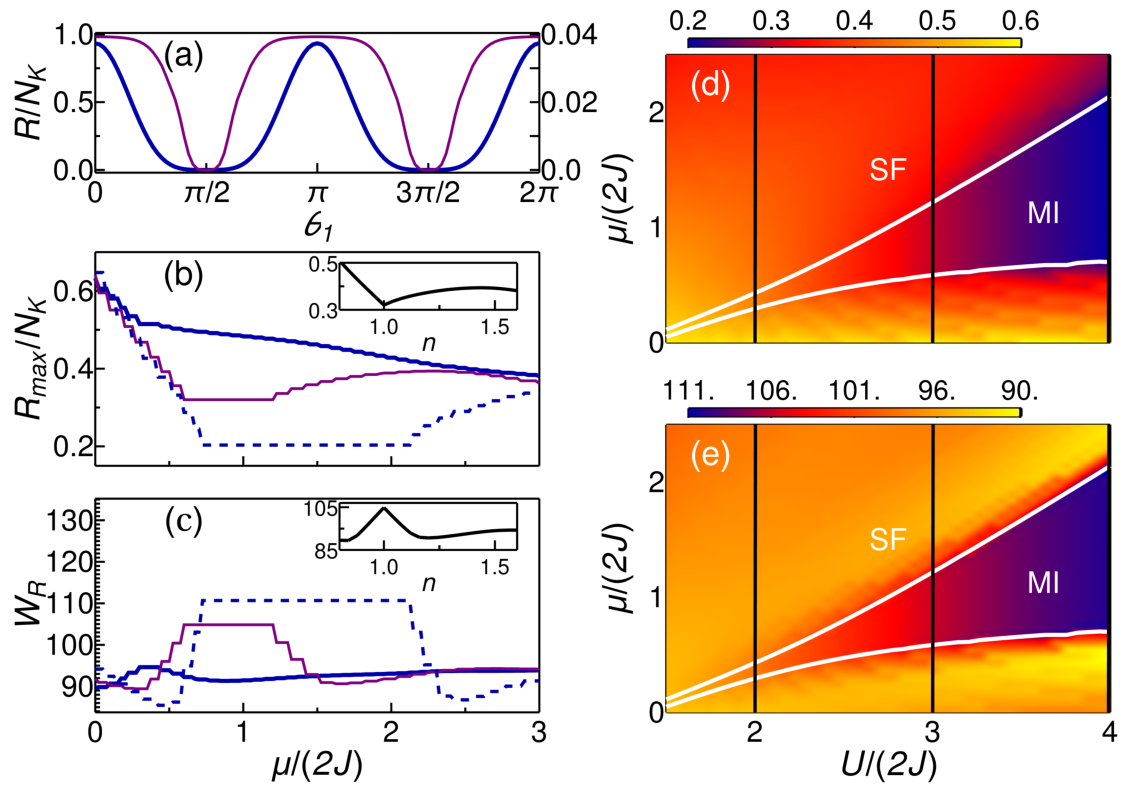
\includegraphics[width=\linewidth]{oph11_3}
  \caption[Mapping the Bose-Hubbard Phase Diagram]{(a) The angular
    dependence of scattered light $R$ for a superfluid (thin purple,
    left scale, $U/2J = 0$) and Mott insulator (thick blue, right
    scale, $U/2J =10$). The two phases differ in both their value of
    $R_\text{max}$ as well as $W_R$ showing that density correlations
    in the two phases differ in magnitude as well as extent. Light
    scattering maximum $R_\text{max}$ is shown in (b, d) and the width
    $W_R$ in (c, e).  It is very clear that varying chemical potential
    $\mu$ or density $\langle n\rangle$ sharply identifies the
    superfluid-Mott insulator transition in both quantities. (b) and
    (c) are cross-sections of the phase diagrams (d) and (e) at
    $U/2J=2$ (thick blue), 3 (thin purple), and 4 (dashed
    blue). Insets show density dependencies for the $U/(2 J) = 3$
    line. $K=M=N=25$.}
	\label{fig:SFMI}
\end{figure}

We then consider probing these ground states using our optical scheme
and we calculate the ``quantum addition'', $R$, based on these ground
states. The angular dependence of $R$ for a Mott insulator and a
superfluid is shown in Fig. \ref{fig:SFMI}(a), and we note that there
are two variables distinguishing the states. Firstly, maximal $R$,
$R_\text{max} \propto \sum_i \langle \delta \hat{n}_i^2 \rangle$,
probes the fluctuations and compressibility $\kappa'$
($\langle \delta \hat{n}^2_i \rangle \propto \kappa' \langle \hat{n}_i
\rangle$).  The Mott insulator is incompressible and thus will have
very small on-site fluctuations and it will scatter little light
leading to a small $R_\text{max}$. The deeper the system is in the
insulating phase (i.e. the larger the $U/2J$ ratio is), the smaller
these values will be until ultimately it will scatter no light at all
in the $U \rightarrow \infty$ limit. In Fig. \ref{fig:SFMI}(a) this
can be seen in the value of the peak in $R$. The value $R_\text{max}$
in the superfluid phase ($U/2J = 0$) is larger than its value in the
Mott insulating phase ($U/2J = 10$) by a factor of
$\sim$25. Figs. \ref{fig:SFMI}(b,d) show how the value of
$R_\text{max}$ changes across the phase transition. There are a few
things to note at this point. Firstly, if we follow the transition
along the line corresponding to commensurate filling (i.e.~any line
that is in between the two white lines in Fig. \ref{fig:SFMI}(d)) we
see that the transition is very smooth and it is hard to see a
definite critical point. This is due to the energy gap closing
exponentially slowly which makes precise identification of the
critical point extremely difficult. The best option at this point
would be to fit Tomonaga-Luttinger theory to the results in order to
find this critical point. However, we note that there is a drastic
change in signal as the chemical potential (and thus the density) is
varied. This is highlighted in Fig. \ref{fig:SFMI}(b) which shows how
the Mott insulator can be easily identified by a dip in the quantity
$R_\text{max}$.

Secondly, being a Fourier transform, the width $W_R$ of the dip in $R$
is a direct measure of the correlation length $l$, $W_R \propto
1/l$. The Mott insulator being an insulating phase is characterised by
exponentially decaying correlations and as such it will have a very
large $W_R$. On the other hand, the superfluid in 1D exhibits pseudo
long-range order which manifests itself in algebraically decaying
two-point correlations \cite{giamarchi} which significantly reduces
the dip in the $R$. This can be seen in
Fig. \ref{fig:SFMI}(a). Furthermore, just like for $R_\text{max}$ we
see that the transition is much sharper as $\mu$ is varied. This is
shown in Figs. \ref{fig:SFMI}(c,e). Notably, the difference in angle
between a superfluid and an insulating state is fairly significant
$\sim 20^\circ$ which should make the two phases easy to identify
using this measure. In this particular case, measuring $W_R$ in the
Mott phase is not very practical as the insulating phase does not
scatter light (small $R_\mathrm{max}$). The phase transition
information is easier extracted from $R_\mathrm{max}$. However, this
is not always the case and we will shortly see how certain phases of
matter scatter a lot of light and can be distinguished using
measurements of $W_R$ where $R_\mathrm{max}$ is not
sufficient. Another possible concern with experimentally measuring
$W_R$ is that it might be obstructed by the classical diffraction
maxima which appear at angles corresponding to the minima in
$R$. However, the width of such a peak is much smaller as its width is
proportional to $1/M$.

So far both variables we considered, $R_\text{max}$ and $W_R$, provide
similar information. They both take on values at one of its extremes
in the Mott insulating phase and they change drastically across the
phase transition into the superfluid phase. Next, we present a case
where it is very different. We will again consider ultracold bosons in
an optical lattice, but this time we introduce some disorder. We do
this by adding an additional periodic potential on top of the exisitng
setup that is incommensurate with the original lattice. The resulting
Hamiltonian can be shown to be
\begin{equation}
  \hat{H}_\mathrm{dis} = -J \sum_{\langle i, j \rangle}
  \bd_i b_j + \frac{U}{2} \sum_i \hat{n}_i (\hat{n}_i - 1) +
  \frac{V}{2} \sum_i \left[ 1 + \cos (2 r \pi m + 2 \phi) \right]
  \hat{n}_i,
\end{equation}
where $V$ is the strength of the superlattice potential, $r$ is the
ratio of the superlattice and trapping wave vectors and $\phi$ is some
phase shift between the two lattice potentials \cite{roux2008}. The
first two terms are the standard Bose-Hubbard Hamiltonian and the only
modification is an additional spatially varying potential shift. We
will only consider the phase diagram at fixed density as the
introduction of disorder makes the usual interpretation of the phase
diagram in the ($\mu/2J$, $U/2J$) plane for a
fixed ratio $V/U$ complicated due to the presence of multiple
compressible and incompressible phases between successive Mott
insulator lobes \cite{roux2008}. Therefore, the chemical potential no
longer appears in the Hamiltonian as we are no longer considering the
grand canonical ensemble.

The reason for considering such a system is that it introduces a
third, competing phase, the Bose glass into our phase diagram. It is
an insulating phase like the Mott insulator, but it has local
superfluid susceptibility making it compressible. Therefore this
localized insulating phase has exponentially decaying correlations
just like the Mott phase, but it has large on-site fluctuations just
like the compressible superfluid phase. As these are the two physical
variables encoded in $R$ measuring both $R_\text{max}$ and $W_R$ will
provide us with enough information to distinguish all three phases. In
a Bose glass we have finite compressibility, but exponentially
decaying correlations. This gives a large $R_\text{max}$ and a large
$W_R$. A Mott insulator also has exponentially decaying correlations
since it is an insulator, but it is incompressible. Thus, it will
scatter light with a small $R_\text{max}$ and large $W_R$. Finally, a
superfluid has long-range correlations and large compressibility which
results in a large $R_\text{max}$ and a small $W_R$.

\begin{figure}  
  \centering
  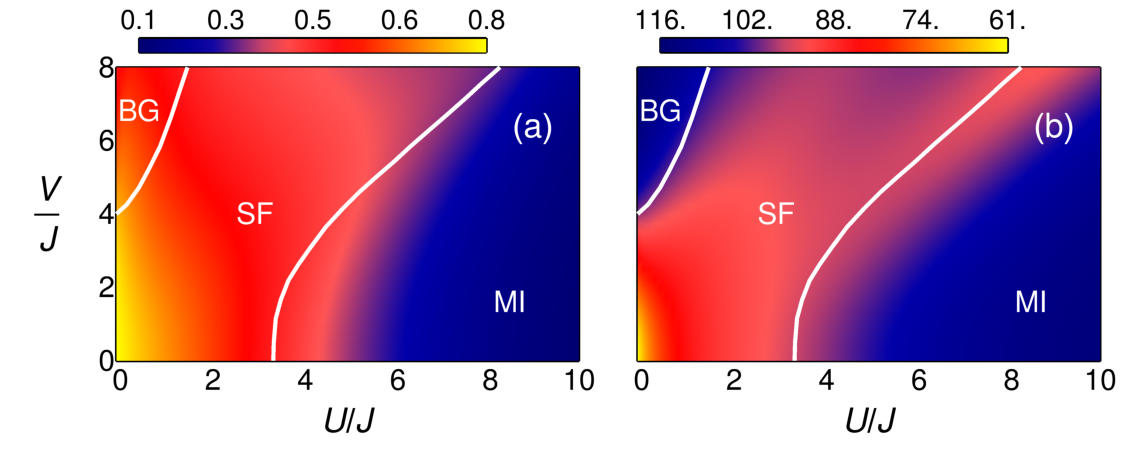
\includegraphics[width=\linewidth]{oph22_3}
  \caption[Mapping the Disoredered Phase Diagram]{The
    Mott-superfluid-glass phase diagrams for light scattering maximum
    $R_\text{max}/N_K$ (a) and width $W_R$ (b). Measurement of both
    quantities distinguish all three phases. Transition lines are
    shifted due to finite size effects \cite{roux2008}, but it is
    possible to apply well known numerical methods to extract these
    transition lines from such experimental data extracted from $R$
    \cite{ejima2011}. $K=M=N=35$.}
  \label{fig:BG}
\end{figure}

We confirm this in Fig. \ref{fig:BG} for simulations with the ratio of
superlattice- to trapping lattice-period $r\approx 0.77$ for various
disorder strengths $V$ \cite{roux2008}. From Fig. \ref{fig:BG} we see
that all three phases can indeed be distinguished. From the
$R_\mathrm{max}$ plot we can distinguish the two compressible phases,
the superfluid and Bose glass, from the incompressible phase, the Mott
insulator. We can now also distinguish the Bose glass phase from the
superfluid, because only one of them is an insulator and thus the
angular width of their scattering patterns will reveal this
information. However, unlike the Mott insulator, the Bose glass
scatters a lot of light (large $R_\mathrm{max}$) enabling such
measurements. Since we performed these calculations at a fixed density
the Mott to superfluid phase transition is not particularly sharp
\cite{cazalilla2011, ejima2011, kuhner2000, pino2012, pino2013} just
like we have seen in Figs. \ref{fig:SFMI}(d,e) if we follow the
transition through the tip of the lobe which corresponds to a line of
unit density. However, despite the lack of an easily distinguishable
critical point, as we have already discussed, it is possible to
quantitatively extract the location of the transition lines by
extracting the Tomonaga-Luttinger parameter from the scattered light,
$R$, in the same way it was done for an unperturbed Bose-Hubbard model
\cite{ejima2011}.

\section{Matter-field interference measurements}

We have shown in section \ref{sec:B} that certain optical arrangements
lead to a different type of light-matter interaction where coupling is
maximised in between lattice sites rather than at the sites themselves
yielding $\a_1 = C\hat{B}$. This leads to the optical fields
interacting directly with the interference terms $\bd_i b_{i+1}$ via
the operator $\hat{B}$ given by Eq. \eqref{eq:B}. This opens up a
whole new way of probing and interacting with a quantum gas trapped in
an optical lattice as this gives an in-situ method for probing the
inter-site interference terms at its shortest possible distance,
i.e.~the lattice period.

Unlike in the previous sections, here we will use the mean-field
description of the Bose-Hubbard model in order to obtain a simple
physical picture of what information is contained in the quantum
light. In the mean-field approximation the inter-site interference
terms become
\begin{equation}
  \bd_i b_j = \Phi \bd_i + \Phi^* b_j - |\Phi|^2,
\end{equation}
where $\langle b_i \rangle = \Phi$ which we assume is uniform across
the whole lattice. This approach has the advantage that the quantity
$\Phi$ is the mean-field order parameter of the superfluid to Mott
insulator phase transition and is effectively a good measure of the
superfluid character of the quantum ground state. This greatly
simplifies the physical interpretation of our results.

Firstly, we will show that our nondestructive measurement scheme
allows one to probe the mean-field order parameter, $\Phi$,
directly. Normally, this is achieved by releasing the trapped gas and
performing a time-of-flight measurement. Here, this can be achieved
in-situ. In section \ref{sec:B} we showed that one of the possible
optical arrangement leads to a diffraction maximum with the matter
operator
\begin{equation}
  \label{eq:Bmax}
  \hat{B}_\mathrm{max} = J^B_\mathrm{max} \sum_i \left( \bd_i b_{i+1}
    + b_i \bd_{i+1} \right),
\end{equation}
where $J^B_\mathrm{max} = \mathcal{F}[W_1](2\pi/d)$. Therefore, by measuring the
expectation value of the quadrature we obtain the following quantity
\begin{equation}
  \langle \hat{X}^F_{\beta=0} \rangle = J^B_\mathrm{max} (K-1) | \Phi |^2 .
\end{equation}
This quantity is directly proportional to square of the order
parameter $\Phi$ and thus lets us very easily follow this quantity
across the phase transition with a very simple quadrature measurement
setup. 

In the mean-field treatment, the order parameter also lets us deduce a
different quantity, namely matter-field quadratures
$\hat{X}^b_\alpha = (b e^{-i\alpha} + \bd e^{i\alpha})/2$. Quadrature
measurements of optical fields are a standard and common tool in
quantum optics. However, this is not the case for matter-fields as
normally most interactions lead to an effective coupling with the
density as we have seen in the previous sections. Therefore, such
measurements provide us with new opportunities to study the quantum
matter state which was previously unavailable. We will take $\Phi$ to
be real which in the standard Bose-Hubbard Hamiltonian can be selected
via an inherent gauge degree of freedom in the order parameter. Thus,
the quadratures themself straightforwardly become
\begin{equation}
  \hat{X}^b_\alpha = \frac{\Phi}{2} (e^{-i\alpha} + e^{i\alpha}) =
  \Phi \cos(\alpha).
\end{equation}
From our measurement of the light field quadrature we have already
obtained the value of $\Phi$ and thus we immediately also know the
values of the matter-field quadratures. Unfortunately, the variance of
the quadrature is a more complicated quantity given by
\begin{equation} 
  (\Delta X^b_{0,\pi/2})^2 = \frac{1}{4} + [(n - \Phi^2) \pm
  \frac{1}{2}(\langle b^2 \rangle - \Phi^2)],
\end{equation} 
where we have arbitrarily selected two orthogonal quadratures
$\alpha =0 $ and $\alpha = \pi / 2$. This quantity cannot be estimated
from light quadrature measurements alone as we do not know the value
of $\langle b^2 \rangle$. To obtain the value of
$\langle b^2 \rangle$this quantity we need to consider a second-order
light observable such as light intensity. However, in the diffraction
maximum this signal will be dominated by a contribution proportional
to $K^2 \Phi^4$ whereas the terms containing information on
$\langle b^2 \rangle$ will only scale as $K$. Therefore, it would be
difficult to extract the quantity that we need by measuring in the
difraction maximum.

\begin{figure}
  \centering
  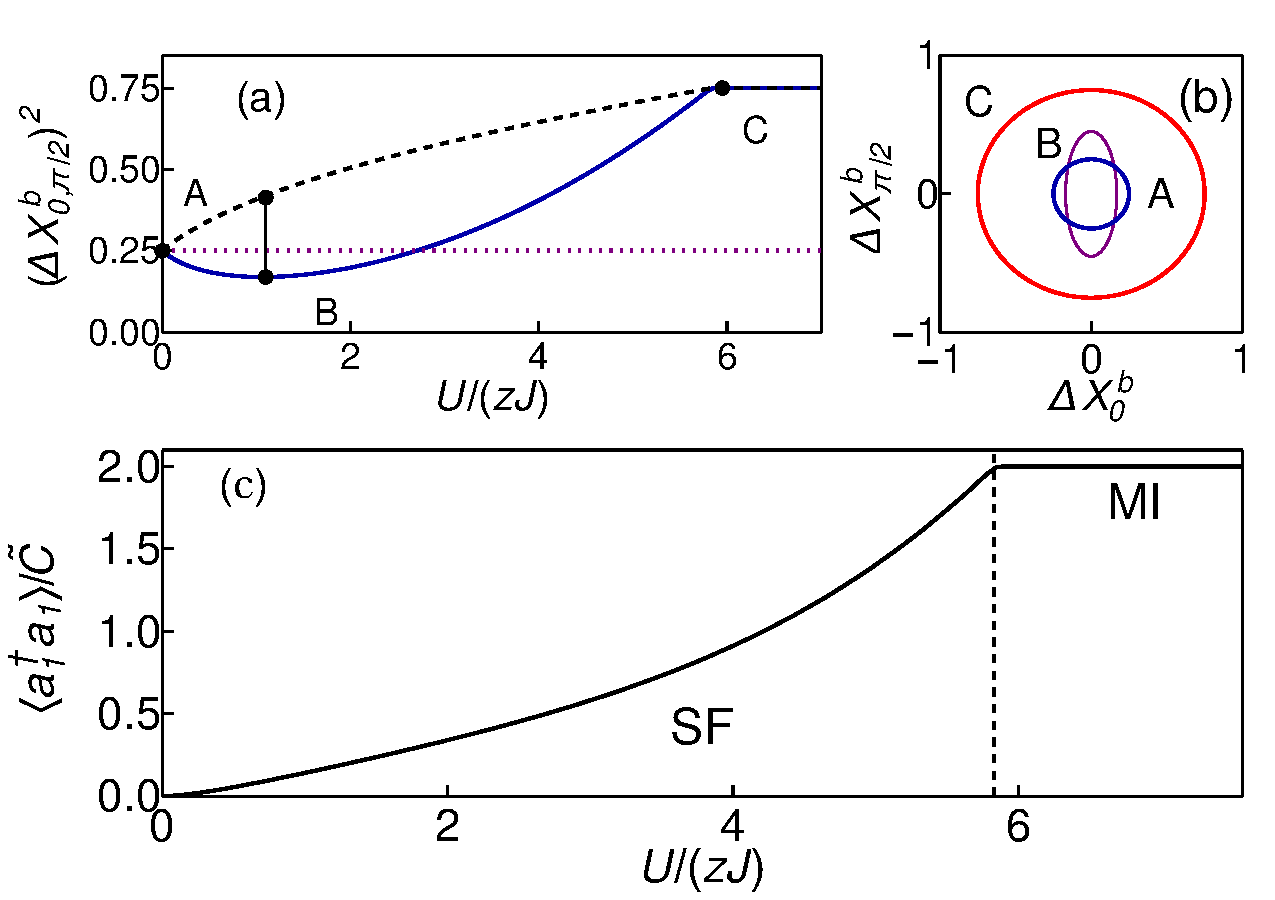
\includegraphics[width=\linewidth]{QuadsC}
  \caption[Mean-Field Matter Quadratures]{Mean-field quadratures and
    resulting photon scattering rates. (a) The variances of
    quadratures $\Delta X^b_0$ (solid) and $\Delta X^b_{\pi/2}$
    (dashed) of the matter field across the phase transition. Level
    1/4 is the minimal (Heisenberg) uncertainty. There are three
    important points along the phase transition: the coherent state
    (SF) at A, the amplitude-squeezed state at B, and the Fock state
    (MI) at C. (b) The uncertainties plotted in phase space. (c)
    Photon number scattered in a diffraction minimum, given by
    Eq. (\ref{intensity}), where
    $\tilde{C} = 2 |C|^2 (K-1) \mathcal{F}^2 [W_1](\pi/d)$.  More
    light is scattered from a MI than a SF due to the large
    uncertainty in phase in the insulator.}
	\label{Quads}
\end{figure}

We now consider the alternative arrangement in which we probe the
diffraction minimum and the matter operator is given by
\begin{equation}
  \label{eq:Bmin}
  \hat{B} = J^B_\mathrm{min} \sum_i (-1)^i \left( \bd_i b_{i+1} b_i
    \bd_{i+1} \right),
\end{equation}
where $J^B_\mathrm{min} = - \mathcal{F}[W_1](\pi / d)$ and which
unlike the previous case is no longer proportional to the Bose-Hubbard
kinetic energy term. Unlike in the diffraction maximum the light
intensity in the diffraction minimum does not have the term
proportional to $K^2$ and thus we obtain the following quantity
\begin{equation}
  \label{intensity}
  \langle \ad_1 \a_1 \rangle = 2 |C|^2(K-1) \mathcal{F}^2[W_1]
  (\frac{\pi}{d}) [ ( \langle b^2 \rangle - \Phi^2 )^2 + ( n - \Phi^2 ) ( 1 +n - \Phi^2 ) ],
\end{equation}
This is plotted in Fig. \ref{Quads} as a function of
$U/(zJ)$. Now, we can easily deduce the value of
$\langle b^2 \rangle$ since we will already know the mean density,
$n$, from our experimental setup and we have seen that we can obtain
$\Phi^2$ from the diffraction maximum. Thus, we now have access to the
quadrature variance of the matter-field as well giving us a more
complete picture of the matter-field amplitude than previously
possible.

A surprising feature seen in Fig. \ref{Quads} is that the inter-site
terms scatter more light from a Mott insulator than a superfluid
Eq. \eqref{intensity}, although the mean inter-site density
$\langle \hat{n}(\b{r})\rangle $ is tiny in the Mott insulating
phase. This reflects a fundamental effect of the boson interference in
Fock states. It indeed happens between two sites, but as the phase is
uncertain, it results in the large variance of $\hat{n}(\b{r})$
captured by light as shown in Eq. \eqref{intensity}. The interference
between two macroscopic BECs has been observed and studied
theoretically \cite{horak1999}. When two BECs in Fock states interfere
a phase difference is established between them and an interference
pattern is observed which disappears when the results are averaged
over a large number of experimental realizations. This reflects the
large shot-to-shot phase fluctuations corresponding to a large
inter-site variance of $\hat{n}(\b{r})$. By contrast, our method
enables the observation of such phase uncertainty in a Fock state
directly between lattice sites on the microscopic scale in-situ.

More generally, beyond mean-field, probing $\hat{B}^\dagger \hat{B}$
via light intensity measurements gives us access with 4-point
correlations ($\bd_i b_j$ combined in pairs). Measuring the photon
number variance, which is standard in quantum optics, will lead up to
8-point correlations similar to 4-point density correlations
\cite{mekhov2007pra}. These are of significant interest, because it
has been shown that there are quantum entangled states that manifest
themselves only in high-order correlations \cite{kaszlikowski2008}.

\section{Conclusions}

In this chapter we explored the possibility of nondestructively
probing a quantum gas trapped in an optical lattice using quantised
light. Firstly, we showed that the density term in scattering has an
angular distribution richer than classical diffraction, derived
generalized Bragg conditions, and estimated parameters for two
relevant experiments \cite{miyake2011, weitenberg2011}. Secondly, we
demonstrated how the method accesses effects beyond mean-field and
distinguishes all the phases in the Mott-superfluid-glass transition,
which is currently a challenge \cite{derrico2014}. Finally, we looked
at measuring the matter-field interference via the operator $\hat{B}$
by concentrating light between the sites. This corresponds to probing
interference at the shortest possible distance in an optical
lattice. This is in contrast to standard destructive time-of-flight
measurements which deal with far-field interference. This quantity
defines most processes in optical lattices. E.g. matter-field phase
changes may happen not only due to external gradients, but also due to
intriguing effects such quantum jumps leading to phase flips at
neighbouring sites and sudden cancellation of tunnelling
\cite{vukics2007}, which should be accessible by our method. We showed
how in mean-field, one can measure the matter-field amplitude (order
parameter), quadratures and squeezing. This can link atom optics to
areas where quantum optics has already made progress, e.g., quantum
imaging \cite{golubev2010, kolobov1999}, using an optical lattice as
an array of multimode nonclassical matter-field sources with a high
degree of entanglement for quantum information processing. Since our
scheme is based on off-resonant scattering, and thus being insensitive
to a detailed atomic level structure, the method can be extended to
molecules \cite{LP2013}, spins, and fermions \cite{ruostekoski2009}.

